\section{Geometria de Uma e Duas Câmeras}

\subsection{Notação Básica de Geometria Projetiva}

Nesta seção, faremos uma breve introdução aos conceitos básicos de Geometria Projetiva e usaremos a notação contida em (citar hartley), por ser o tipo de notação mais difundido entre pesquisas de visão computacional. Para uma abordagem mais profunda do assunto o leitor pode pesquisar o referido autor.  

\subsubsection{O Espaço Projetivo em Duas Dimensões}



$\Longrightarrow$ A Reta


Sabemos que uma reta no plano $\mathbb{R}^{2}$ pode ser representada pela equação $a\,x+b\,y+c=0$, onde a reta fica perfeitamente determinada pelos valores das constantes $a,b,c$. Desta forma, podemos representar retas através de vetores, e assim a reta $a\,x+b\,y+c=0$ seria representada por $(a,b,c)^T \in \mathbb{R}^{3}$, utlizando o símbolo em negrito $\lightrgb$ para indicar tal vetor escrito em coluna, por padrão. Portanto $\lightrgb = (a,b,c)^T$. Note que a relação entre uma dada reta e o seu respectivo vetor não é biunívoca, pois o vetor $k\,(a,b,c)^T$, tal que $k \in \mathbb{R}$, representa a reta $k\,a\,x+k\,b\,y+k\,c=0$ que é a mesma reta $a\,x+b\,y+c=0$. Temos, então, infinitos vetores (chamados paralelos na Álgebra Linear) que representam uma mesma reta e formam uma classe de equivalência, onde essa classe pode ser repsentada por qualquer um de seus vetores. Os vetores de uma classe de equivalência, definida pela multiplicação por um escalar, são conhecidos como vetores {\it homogêneos}. O conjunto de classes de equivalência de vetores em $\mathbb{R}^{3} - (0,0,0)^T$ forma o {\it Espaço Projetivo} $\mathbb{P}^{2}$. O vetor $(0,0,0)^T$ foi excluído por não representar reta alguma. Após essas considerações, dizemos que uma reta no plano é representada pelo vetor $(a,b,c)^T$ em {\it coordenadas homogêneas}.
\\

$\Longrightarrow$ O Ponto


Sabemos também, que em $\mathbb{R}^{2}$ os pontos são representados através de pares ordenados do tipo $(x,y)$, assim cada ponto pode ser identificado como um vetor $(x,y)^T$. Os vetores que se referem a pontos serão representados pelo símbolo em negrito $\x$, que sempre indicará um vetor coluna. Desse jeito, $\x=(x,y)^T$. Sabemos também que um ponto $(x,y)^T$ pertence a uma reta $(a,b,c)^T$ se, e somente se $a\,x+b\,y+c=0$, e podemos realizar essa verificação utilizando multiplicação matricial, escrevendo $\x$ com uma terceira coordenada igual a 1:

\begin{center}
$\begin{array}{ccccc}
 (x,y,1)^T 
&\begin{pmatrix}
 a  \\ 
 b  \\ 
 c 
 \end{pmatrix} 
& = 0 \qquad 
& \text{ou} 
& \qquad \x ^T\lightrgb = 0.
\end{array}$
\end{center}

Ou seja, temos um ponto de $\mathbb{R}^{2}$ representado como um vetor com três coordenadas. Observe que para $k \in \mathbb{R} - \{0\}$, temos:

\begin{center}
$\begin{array}{ccccccc}
 (k\,x,k\,y,k)^T 
&\begin{pmatrix}
 a  \\ 
 b  \\ 
 c 
 \end{pmatrix} 
& = 0
& \qquad \leftrightarrow \qquad
& (x,y,1)^T
&\begin{pmatrix}
 a  \\ 
 b  \\ 
 c 
 \end{pmatrix} 
& = 0.
\end{array}$
\end{center}

Portanto,  variando $k$, podemos considerar os vetores em coordenadas homogeneas $(k\,x,k\,y,k)^T \in \mathbb{P}^2$, como representantes do mesmo ponto $(x,y)^T \in \mathbb{R}^2$, e podemos resgatar nossa representaçao original aplicando o procedimento $(x/k,y/k)^T$, pois $k \ne 0$.

\begin{figure}[!htb]
\centering
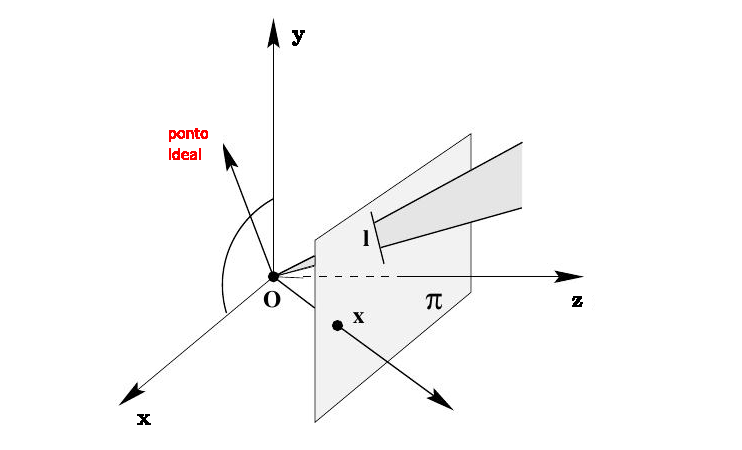
\includegraphics[scale=0.8]{espaco_P2}
\caption{O plano $\pi$ representa o espaço projetivo $\mathbb{P}^2$. Pontos e retas pertencentes a esse espaço são representados, respectivamente, por raios e planos que passam pela origem do $\mathbb{R}^3$.}
\label{plano_P2}
\end{figure}

Podemos pensar no esapaço projetivo como um conjunto de raios passando pela origem do $\mathbb{R}^3$, onde cada raio representa um único ponto, que é a interseção desse raio com o plano $\mathbb{P}^2$. Desta mesma forma, retas em $\mathbb{P}^2$ são formadas por planos. Na figura \ref{plano_P2}, podemos observar com a interseção do raio com o plano define um ponto, assim como a interseção de dois planos definem uma reta.
\\

$\Longrightarrow$ A Cônica


Em geometria Euclidiana, as cônicas são de três tipos principais: elipse, hipérbole e parábola. São definidas, algebricamente, por uma equação do segundo grau em duas variáveis, considerando coordenadas não homogêneas:

\begin{equation*}
a\,x^2+b\,x\,y+c\,y^2+d\,x+e\,y+f=0.
\end{equation*}

Sabemos que um ponto pertence à cônica se ele é solução da equação acima, a qual pode ser representada utilizando multiplicação matricial e vetores em coordenadas homogêneas, com a terceira coordenada configurada como 1:

\begin{center}
$
\begin{array}{cccc}
  (x,y,1)^T 
& \begin{bmatrix}
a & b/2 & d/2\\
b/2 & c & e/2\\
d/2 & e/2 & f
\end{bmatrix}
& \begin{pmatrix}
x\\
y\\
1
\end{pmatrix}
& = 0.
\end{array}
$
\end{center}

Podemos generalizar essas coordenadas homogêneas fazendo as substituições $x = x_{1}/x_{3}$ e $y = x_{2}/x_{3}$, e nossa equação do elípse fica:

\begin{equation*}
a\,x_1^2+b\,x_1\,x_2+c\,x_2^2+d\,x_1\,x_3+e\,x_2\,x_3+f\,x_3^2=0.
\end{equation*}

Novamente em notação matricial:

\begin{center}
$
\begin{array}{cccccc}
  (x_1,x_2,x_3)^T 
& \begin{bmatrix}
  a & b/2 & d/2\\
  b/2 & c & e/2\\
  d/2 & e/2 & f
  \end{bmatrix}
& \begin{pmatrix}
  x_1\\
  x_2\\
  x_3
  \end{pmatrix}
& = 0
& \qquad \text{ou} \qquad
& \x^T\,C\,\x = 0.
\end{array}
$
\end{center}

Já que um ponto pertence à cônica se, e somente se, satisfaz a última equação, temos que $C$ fica definida como a matriz que representa uma cônica no espaço projetivo $\mathbb{P}^2$.

\begin{center}
$
\begin{array}{cc}
C = & \begin{bmatrix}
      a & b/2 & d/2\\
      b/2 & c & e/2\\
      d/2 & e/2 & f
      \end{bmatrix}.
\end{array}
$
\end{center}




\subsubsection{O Espaço Projetivo em Três Dimensões}


$\Longrightarrow$ O Ponto


Analogamente à representação de um ponto no espaço $\mathbb{P}^2$, um ponto no espaço $\mathbb{P}^3$ é repesentado através de coordenadas homogêneas, acrescentando-se uma quarta coordenada ao vetor que representa esse ponto. Desta forma, $\X = (X_1,X_2,X_3,X_4)^T$ e $X_4 \ne 0$, onde $\X$ é a representação em coordenadas homogêneas do ponto $(X,Y,Z)^T \in \mathbb{R}^3$. Para realizar essa mudança basta tomar 

\begin{equation*}
X=X_1/X_4 \,\, ,\, Y=X_2/X_4 \,\,\, \text{e} \,\,\, Z=X_3/X_4.
\end{equation*}


$\Longrightarrow$ O Plano

Temos que a representação algébrica de um plano $\bpi$ no espaço $\mathbb{R}^3$ é dada pela equação

\begin{equation*}
\pi_1\,X+\pi_2\,Y+\pi_3\,Z+\pi_4=0.
\end{equation*}


\subsection{Notação Usada por Fabbri}
Usar figura do artigo.

\subsection{Resumo dos Resultados Fabbri}
Projeção e reconstrução 3D com o uso de tangentes.
